\let\negmedspace\undefined
\let\negthickspace\undefined
\documentclass[journal]{IEEEtran}
\usepackage[a5paper, margin=10mm, onecolumn]{geometry}
\usepackage{lmodern} % Ensure lmodern is loaded for pdflatex
\usepackage{tfrupee} % Include tfrupee package

\setlength{\headheight}{1cm} % Set the height of the header box
\setlength{\headsep}{0mm}     % Set the distance between the header box and the top of the text

\usepackage{gvv-book}
\usepackage{gvv}
\usepackage{cite}
\usepackage{amsmath,amssymb,amsfonts,amsthm}
\usepackage{algorithmic}
\usepackage{graphicx}
\usepackage{textcomp}
\usepackage{xcolor}
\usepackage{txfonts}
\usepackage{listings}
\usepackage{enumitem}
\usepackage{mathtools}
\usepackage{gensymb}
\usepackage{comment}
\usepackage[breaklinks=true]{hyperref}
\usepackage{tkz-euclide} 
\usepackage{listings}
\usepackage{gvv}                                        
\def\inputGnumericTable{}                                 
\usepackage[latin1]{inputenc}                                
\usepackage{color}                                            
\usepackage{array}                                            
\usepackage{longtable}                                       
\usepackage{calc}                                             
\usepackage{multirow}                                         
\usepackage{hhline}                                           
\usepackage{ifthen}                                           
\usepackage{lscape}
\usepackage{tikz}
\usepackage{tcolorbox}
\usetikzlibrary{matrix}
\usepackage{url}
\usepackage{xcolor}
\usepackage{subcaption}

\begin{document}

\bibliographystyle{IEEEtran}
\vspace{3cm}

\title{11.16.3.8.6}
\author{EE24BTECH11005 - Arjun Pavanje}
% \maketitle
% \newpage
% \bigskip
{\let\newpage\relax\maketitle}
\textbf{Question:}\newline
Three coins are tossed once. Find the probability of getting 3 tails \newline
\solution \newline
The sample space $\Omega$ in case of this experiment is given by,
\begin{align}
  \Omega = \cbrak{HHH, HHT, HTH, HTT, THH, THT, TTH, TTT}
\end{align} 
Now we define a discrete random variable $X =$ number of tails in the sequence. In this solution, we treat our random variable $X$ as a sum of three Bernoulli random variables
\begin{align}
 X = X_1 + X_2 + X_3
\end{align}
where,
\begin{align}
  X_i &= \begin{cases}
    0 & i^{th}\text{toss is heads}\\
    1 & i^{th}\text{toss is tails}
  \end{cases}
\end{align}
Here $p = \frac{1}{2}$. Our random variable is a sum of three Bernoulli random variables. By applying $Z$ transform on both sides and applying properties of $Z$ transform of PMF, 
\begin{align}
  M_X\brak{z} = M_{X_1}\brak{z} M_{X_2}\brak{z}M_{X_3}\brak{z} 
\end{align}
Here, the three coin tosses can be considered as independant events, which implies  $ M_{X_1}\brak{z} = M_{X_2}\brak{z} = M_{X_3}\brak{z}$. Because of this, we can generalize this to $m$ coin tosses.
\begin{align}
  M_X\brak{z} = \prod_{k=1}^{m} M_{X_k}\brak{z}
\end{align}
We now define Probability Mass Function for the Bernoulli random variable $X_i$ be given by,
\begin{align}
  p_{X_i}\brak{n} = \begin{cases}
    p & n = 0\\
    1-p & n = 1\\
    0 &  n \in \mathbb{Z} - \cbrak{0,1}
  \end{cases}
\end{align}
where $p$ is the probability of getting heads
\begin{align}
  M_{X_1}\brak{z}&=\sum_{k=-\infty}^{\infty}p_{X_1}\brak{k}z^{-n} = p + \brak{1-p}z^{-1}\\
  M_{X_2}\brak{z}&=\sum_{k=-\infty}^{\infty}p_{X_2}\brak{k}z^{-n} = p + \brak{1-p}z^{-1}\\
  &\vdots\\
  M_{X_m}\brak{z}&=\sum_{k=-\infty}^{\infty}p_{X_m}\brak{k}z^{-n} = p + \brak{1-p}z^{-1}\\   M_X\brak{z} &= \brak{p + \brak{1-p}z^{-1}}^{m}
\end{align}
This can be simplified to,
\begin{align}
  M_X\brak{z} = \sum_{n=-\infty}^{\infty} \comb{m}{k}p^{k}\brak{1-p}^{3-k}z^{-k}
\end{align}
Taking $z-$inverse on both sides we get,
\begin{align}
  p_X\brak{n} = \comb{m}{k} p^{k} \brak{1-p}^{3-k} 
\end{align}
Taking $m=3, p = \frac{1}{2}$ we get,
\begin{align}
  p_X\brak{n} = \comb{3}{n}\brak{\frac{1}{2}}^3
\end{align}
Here, since we require probability of $3$ tails out of $3$ tosses, set $k=3$ in the above equation.\newline
Required probability $=\frac{1}{8}$\newline
If we redefine the problem a little bit, it can be solved using Cummulative Frequency Distribution. We can say $\pr{\text{3 tails}} = 1 - \pr{\text{Atleast one head}}$ since out of three coin tosses there can be at max $3$ tails.\newline
We can say that 
\begin{align}
  \pr{\text{m-k tails}} &= \pr{\text{k heads}}\\
  \pr{\text{atleast k heads}} &= \pr{\text{atleast m-k tails}}
\end{align}
For our problem $m=3, k=1$
Cummulative Distribution Function is given by,
\begin{align}
    F_X \brak{n} = \sum _{k=-\infty}^{n} \comb{3}{k} \brak{\frac{1}{2}}^3\\ 
    F_{X}\brak{n} = \begin{cases}
        0 & \quad n < 0\\
        \comb{3}{0}\brak{\frac{1}{2}}^3 = \frac{1}{8} & \quad 0 \leq n < 1\\
        \comb{3}{0}\brak{\frac{1}{2}}^3 + \comb{3}{1}\brak{\frac{1}{2}}^3 = \frac{1}{2} & \quad 1 \leq n < 2\\
        \comb{3}{0}\brak{\frac{1}{2}}^3 + \comb{3}{1}\brak{\frac{1}{2}}^3 + \comb{3}{2}\brak{\frac{1}{2}}^3 = \frac{7}{8} & \quad 2 \leq n < 3\\
        \comb{3}{0}\brak{\frac{1}{2}}^3 + \comb{3}{1}\brak{\frac{1}{2}}^3 + \comb{3}{2}\brak{\frac{1}{2}}^3 + \comb{3}{3}\brak{\frac{1}{2}}^3 = 1 & \quad 3 \leq n
    \end{cases}
\end{align}
What we require is,
\begin{align}
  1 - \pr{\brak{X \ge 1}} &= 1 - \brak{1 - F_X\brak{1} } \\
   &= \frac{1}{8}
\end{align}

\textbf{Simulation:}\newline
Generating random numbers with uniform probability was done using OpenSSL's rand by the following proccess
\begin{enumerate}
  \item $1$ random byte is generated using OpenSSL's rand. 
  \item The randomly generated number is scaled down from $255$ to between $0$ to $1$ by dividing. 
  \item To generate a Bernoulli Random variable, return 0, if generated number is less than $p$, else return $1$.
\end{enumerate}
\begin{figure}[h!]
  \centering
  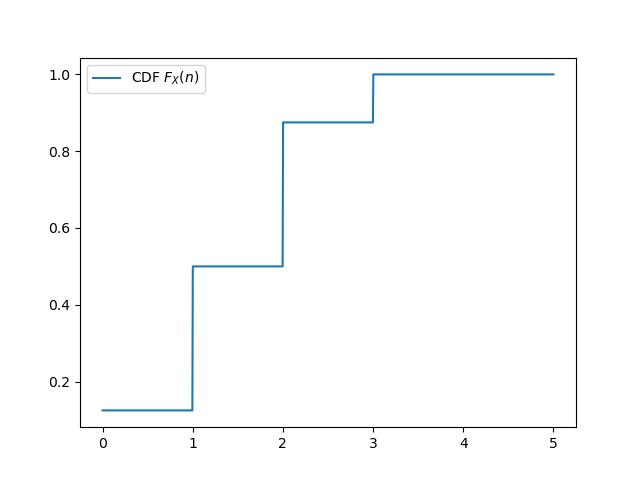
\includegraphics[width=0.7\columnwidth]{figs/cdf.png}
  \caption{CDF Plot}
  \label{label}
\end{figure}

\begin{figure}[h!]
  \centering
  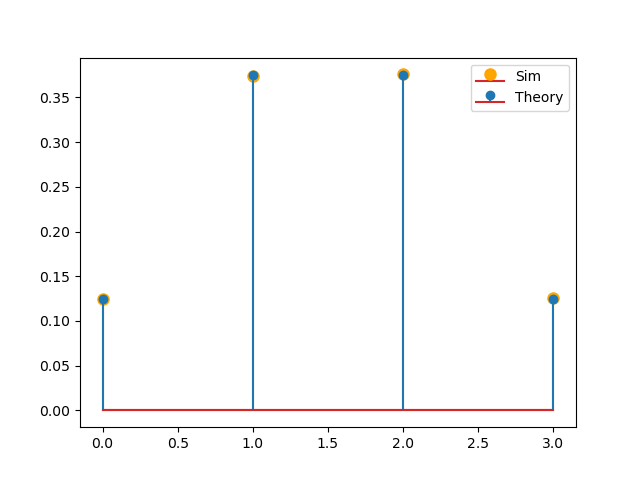
\includegraphics[width=0.7\columnwidth]{figs/pmf_1.png}
  \caption{PMF plot for $m$ = 3}
  \label{label}
\end{figure}

We notice something interesting about PMF plots for different values of $m$. We see that it appears to converge Gaussian Distribution curve. One more interesting fact is that area under the Gaussian Distribution Curve is $1$. This further supports the fact that PMF converges to Gaussian Distribution Curve, as sum of all the probabilites $\brak{\sum P_X\brak{n} = 1}$ is $1$.  As $m \rightarrow \infty$ the PMF plot onverges to the Gaussian Distribution curve. We can visually verify this, \newline

Below are the PMF graphs for $m = 10, 25, 500, 100$ respectively
\begin{figure*}[h!]
    {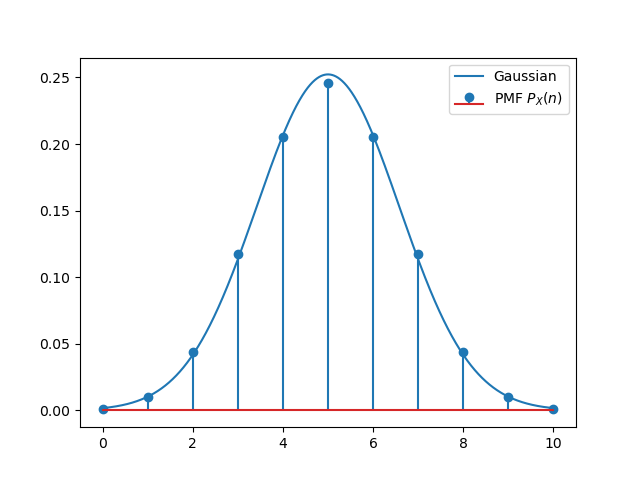
\includegraphics[ width=0.53\columnwidth]{./figs/pmf2.png}}
    \hspace{\fill}
    {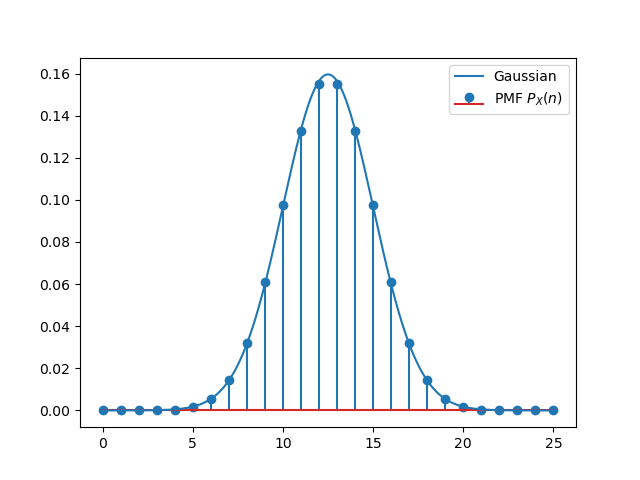
\includegraphics[ width=0.53\columnwidth]{./figs/pmf3.png}}
\end{figure*}

\begin{figure*}[h!]
    {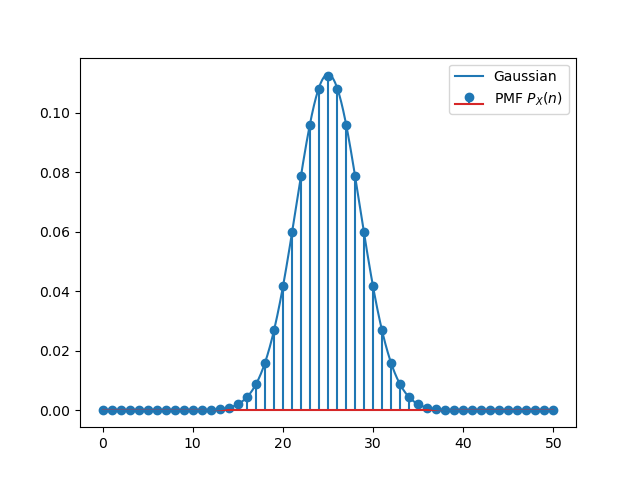
\includegraphics[ width=0.53\columnwidth]{./figs/pmf4.png}}
    \hspace{\fill}
    {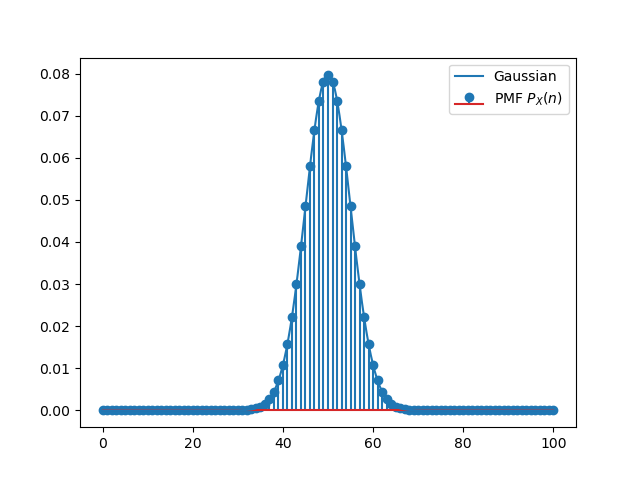
\includegraphics[ width=0.53\columnwidth]{./figs/pmf5.png}}
\end{figure*}
\end{document}
